%!TEX root=../document.tex

\section{Ubuntu Server aufsetzen}
Der erste Schritt war es, die 2 bzw. 3 Server aufzusetzen. Das System besteht aus insgesamt 3 VPS (Virtual Private Server), 2 Nodes (Auch Cluster member genannt) und einem Client der mit dem Cluster interagiert. 

Dafür wurde eine virtuelle Maschine erstellt, auf welcher \verb|ubuntu-14.04.3-server| installiert wurde.
Der Effizienz halber wurde nur eine erstellt und anschließend 2 mal geklont und auf den jeweiligen Maschinen noch die Hostnamen konfiguriert.

\subsection{Nat-Netzwerk}
Das erste Problem war als die 3 Server gestartet wurden, dass die Kommunikation unmöglich war. Das lag daran das jede Maschine lediglich über \verb|NAT| mit dem Host verbunden war, und somit keine Verbindung zwischen den einzelnen VM's bestand.

Um dies zu lösen wurde in Virtualbox ein sogenanntes \verb|NAT-Netzwerk| erstellt, welches den jeweiligen VM's ermöglicht sowohl sich über den Host in das Internet zu verbinden als auch mit den anderen VM's zu kommunizieren. Zusätzlich wird noch ein DHCP Service angeboten, welcher den Maschinen noch eigene IP's automatisch zuweißt. 

\begin{minipage}{\linewidth}
	\centering
	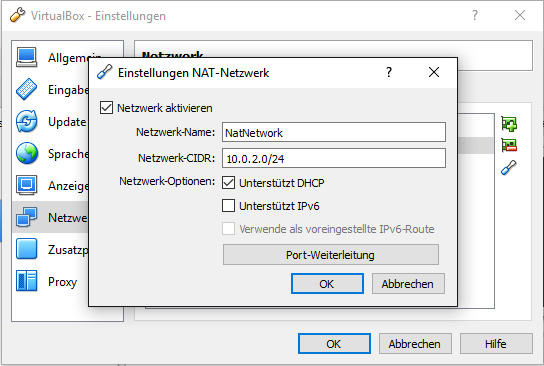
\includegraphics[width=0.53\linewidth]{images/natnetwork}
	\figcaption{Es wurde ein Nat-Netzwerk erstellt mit einem DHCP Server}
\end{minipage}

Nun musste bei den einzelnen VM's noch angegeben werden dass die Netzwerkkarte sich nicht über NAT zu verbinden hat, sondern über unser NatNetwork:

\begin{minipage}{\linewidth}
	\centering
	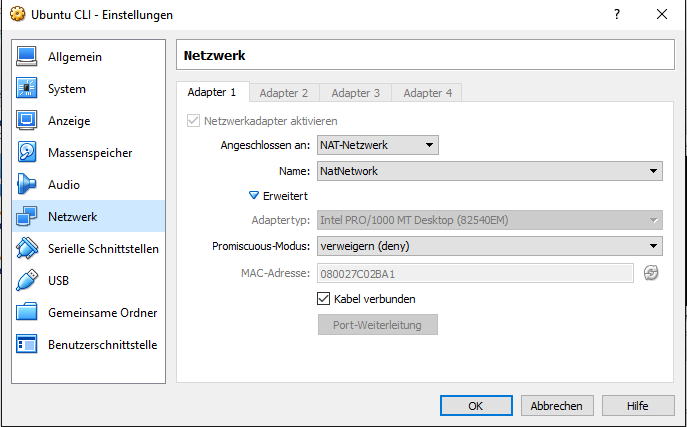
\includegraphics[width=0.6\linewidth]{images/natnetwork2}
	\figcaption{Virtuelle Maschine kommuniziert über Nat-Netzwerk}
\end{minipage}

Ein weiteres skurriles Problem ist in meinem Fall aufgetreten, und zwar ist mir aufgefallen das 2 meiner 3 Virtuellen Maschinen vom DHCP-Server die gleiche IP zugewiesen bekommen haben. Dieses Problem ist aufgetreten da beim klonen der einzelnen VPS' die MAC-Adressen der Netzwerkkarte auch kopiert wurde, und somit hat DHCP angenommen dass dies die gleichen Netzwerkkarten seien. 

\section{DNS Auflösung konfigurieren}
Der erste Schritt war es auf jedem VPS zu definieren, welche Nodes bzw. Clients es gibt die interagieren und was deren IP-Adresse und Name ist. Dazu musste herausgefunden werden welche IP-Adressen die jeweiligen VPS besitzen, dies funktioniert mit dem Befehl \verb|ifconfig|.

Nun das man alle IP-Adressen kennt, werden diese, zusammen mit einem Namen, in das \verb|hosts| file von jedem VPS eingetragen. Die eigene Maschine sollte auch in der Liste sein, die hosts file sollten etwa so aussehene: 

\begin{lstlisting}[language=bash]
:127.0.0.1	localhost
127.0.1.1	Node1
10.0.2.5 Node1.mwoelfer.at Node1
10.0.2.4 Client.mwoelfer.at Client
10.0.2.15 Node2.mwoelfer.at Node2


# The following lines are desirable for IPV6 capable hosts
::1 localhost ip6-localhost ip6-loopback
ff02::1 ip6-allnodes
ff02::2 ip6-allrouters
\end{lstlisting}